% ------------------------------------------------------------------------------------------------------------------
% Basic configuration of Beamera class and Jagiellonian theme
% ------------------------------------------------------------------------------------------------------------------
\RequirePackage[l2tabu, orthodox]{nag}



\ifx\PresentationStyle\notset
  \def\PresentationStyle{dark}
\fi



\documentclass[10pt,t]{beamer}
\mode<presentation>
\usetheme[style=\PresentationStyle,JUlogotitle=no]{jagiellonian}




% ------------------------------------------------------------------------------------
% Procesing configuration files of Jagiellonian theme loceted in directory
% "preambule".
% ------------------------------------------------------------------------------------
% Configuration for polish language
% Need description
\usepackage[polish]{babel}
% Need description
\usepackage[MeX]{polski}



% ------------------------------
% Better support of polish chars in technical parts of PDF
% ------------------------------
\hypersetup{pdfencoding=auto,psdextra}

% Package "textpos" give as enviroment "textblock" which is very usefull in
% arranging text on slides.

% This is standard configuration of "textpos"
\usepackage[overlay,absolute]{textpos}

% If you need to see bounds of "textblock's" comment line above and uncomment
% one below.

% Caution! When showboxes option is on significant ammunt of space is add
% to the top of textblock and as such, everyting put in them gone down.
% We need to check how to remove this bug.

% \usepackage[showboxes,overlay,absolute]{textpos}



% Setting scale length for package "textpos"
\setlength{\TPHorizModule}{10mm}
\setlength{\TPVertModule}{\TPHorizModule}


% ---------------------------------------
% Packages written for lectures "Geometria 3D dla twórców gier wideo"
% ---------------------------------------
% \usepackage{./Geometry3DPackages/Geometry3D}
% \usepackage{./Geometry3DPackages/Geometry3DIndices}
% \usepackage{./Geometry3DPackages/Geometry3DTikZStyle}
% \usepackage{./ProgramowanieSymulacjiFizykiPaczki/ProgramowanieSymulacjiFizykiTikZStyle}
% \usepackage{./Geometry3DPackages/mathcommands}


% ---------------------------------------
% TikZ
% ---------------------------------------
% Importing TikZ libraries
\usetikzlibrary{arrows.meta}
\usetikzlibrary{positioning}





% % Configuration package "bm" that need for making bold symbols
% \newcommand{\bmmax}{0}
% \newcommand{\hmmax}{0}
% \usepackage{bm}




% ---------------------------------------
% Packages for scientific texts
% ---------------------------------------
% \let\lll\undefined  % Sometimes you must use this line to allow
% "amsmath" package to works with packages with packages for polish
% languge imported
% /preambul/LanguageSettings/JagiellonianPolishLanguageSettings.tex.
% This comments (probably) removes polish letter Ł.
\usepackage{amsmath}  % Packages from American Mathematical Society (AMS)
\usepackage{amssymb}
\usepackage{amscd}
\usepackage{amsthm}
\usepackage{siunitx}  % Package for typsetting SI units.
\usepackage{upgreek}  % Better looking greek letters.
% Example of using upgreek: pi = \uppi


\usepackage{calrsfs}  % Zmienia czcionkę kaligraficzną w \mathcal
% na ładniejszą. Może w innych miejscach robi to samo, ale o tym nic
% nie wiem.










% ---------------------------------------
% Packages written for lectures "Geometria 3D dla twórców gier wideo"
% ---------------------------------------
% \usepackage{./ProgramowanieSymulacjiFizykiPaczki/ProgramowanieSymulacjiFizyki}
% \usepackage{./ProgramowanieSymulacjiFizykiPaczki/ProgramowanieSymulacjiFizykiIndeksy}
% \usepackage{./ProgramowanieSymulacjiFizykiPaczki/ProgramowanieSymulacjiFizykiTikZStyle}





% !!!!!!!!!!!!!!!!!!!!!!!!!!!!!!
% !!!!!!!!!!!!!!!!!!!!!!!!!!!!!!
% EVIL STUFF
\if\JUlogotitle1
\edef\LogoJUPath{LogoJU_\JUlogoLang/LogoJU_\JUlogoShape_\JUlogoColor.pdf}
\titlegraphic{\hfill\includegraphics[scale=0.22]
{./JagiellonianPictures/\LogoJUPath}}
\fi
% ---------------------------------------
% Commands for handling colors
% ---------------------------------------


% Command for setting normal text color for some text in math modestyle
% Text color depend on used style of Jagiellonian

% Beamer version of command
\newcommand{\TextWithNormalTextColor}[1]{%
  {\color{jNormalTextFGColor}
    \setbeamercolor{math text}{fg=jNormalTextFGColor} {#1}}
}

% Article and similar classes version of command
% \newcommand{\TextWithNormalTextColor}[1]{%
%   {\color{jNormalTextsFGColor} {#1}}
% }



% Beamer version of command
\newcommand{\NormalTextInMathMode}[1]{%
  {\color{jNormalTextFGColor}
    \setbeamercolor{math text}{fg=jNormalTextFGColor} \text{#1}}
}


% Article and similar classes version of command
% \newcommand{\NormalTextInMathMode}[1]{%
%   {\color{jNormalTextsFGColor} \text{#1}}
% }




% Command that sets color of some mathematical text to the same color
% that has normal text in header (?)

% Beamer version of the command
\newcommand{\MathTextFrametitleFGColor}[1]{%
  {\color{jFrametitleFGColor}
    \setbeamercolor{math text}{fg=jFrametitleFGColor} #1}
}

% Article and similar classes version of the command
% \newcommand{\MathTextWhiteColor}[1]{{\color{jFrametitleFGColor} #1}}





% Command for setting color of alert text for some text in math modestyle

% Beamer version of the command
\newcommand{\MathTextAlertColor}[1]{%
  {\color{jOrange} \setbeamercolor{math text}{fg=jOrange} #1}
}

% Article and similar classes version of the command
% \newcommand{\MathTextAlertColor}[1]{{\color{jOrange} #1}}





% Command that allow you to sets chosen color as the color of some text into
% math mode. Due to some nuances in the way that Beamer handle colors
% it not work in all cases. We hope that in the future we will improve it.

% Beamer version of the command
\newcommand{\SetMathTextsColor}[2]{%
  {\color{#1} \setbeamercolor{math text}{fg=#1} #2}
}


% Article and similar classes version of the command
% \newcommand{\SetMathTextColor}[2]{{\color{#1} #2}}










% ---------------------------------------
% Commands for setting background pictures for some slides
% ---------------------------------------
\newcommand{\TitleBackgroundPicture}
{./PresentationPictures/CommonPictures/Cute_dragon_BG_dark.png}
\newcommand{\SectionBackgroundPicture}
{./PresentationPictures/CommonPictures/Cute_dragon_small_BG_light.png}



\newcommand{\TitleSlideWithPicture}{
  \begingroup

  \usebackgroundtemplate{ % \hspace*{-11.5em}
    \includegraphics[height=\paperheight]{\TitleBackgroundPicture}}

  \maketitle

  \endgroup
}





\newcommand{\SectionSlideWithPicture}[1]{%
  \begingroup

  \usebackgroundtemplate{ % \hspace*{-11.5em}
    \includegraphics[height=\paperheight]{\SectionBackgroundPicture}}

  \setbeamercolor{titlelike}{fg=normal text.fg}

  \section{#1}

  \endgroup
}





\newcommand{\EndingSlide}[1]{%
  \begin{frame}[standout]

    \begingroup

    \color{jFrametitleFGColor}

    #1

    \endgroup

  \end{frame}
}










% ------------------------------------------------------
% BibLaTeX
% ------------------------------------------------------
% Package biblatex, with biber as its backend, allow us to handle
% bibliography entries that use Unicode symbols outside ASCII.
\usepackage[
language=polish,
backend=biber,
style=alphabetic,
url=false,
eprint=true,
]{biblatex}

\addbibresource{SystemyOperacyjneBibliography.bib}





% ------------------------------------------------------
% Importing packages, libraries and setting their configuration.
% ------------------------------------------------------





% ------------------------------------------------------
% Special configuration for this particular presentation.
% ------------------------------------------------------










% ------------------------------------------------------------------------------------------------------------------
\title{Systemy operacyjne}
\subtitle{Wprowadzenie do systemu GNU/Linux}

\author{Kamil Ziemian}


% \date{}
% ------------------------------------------------------------------------------------------------------------------










% ####################################################################
% Beginning of the document
\begin{document}
% ####################################################################





% ######################################
% Text is adjusted to the left and words are broken at the end of the line.
% Number of chars: 62k+, 12k+, 20k+, 27k+, 24k+,
\RaggedRight
% ######################################





% ######################################
\maketitle
% ######################################





% ##################
\begin{frame}
  \frametitle{Spis treści}


  \tableofcontents

\end{frame}
% ##################





% ######################################
\section{Informacje ogólne}
% ######################################



% ##################
\begin{frame}
  \frametitle{Informacje wstępne}


  Obawiam~się, że na tych konkretnych zajęciach będzie sporo przynudzania,
  ale nie widzę sposobu, jak tego uniknąć.

  Według mnie to zajęcia są dla studentów, nie studenci dla zajęć. Tak samo
  ja tu jestem dla Państwa, a~nie Państwo dla mnie. W~związku z~tym, ja nie
  będę Państwa rozliczał z~obecności na zajęciach, tylko z~wiedzy
  i~umiejętności. Jeśli uważają Państwo, że~są lepsze rzeczy do robienia,
  niż bycie na tych zajęciach, w~to mi graj.

  \textbf{Pytanie.} Kto z~Państwa \textit{nie} używa na codzień systemu
  operacyjnego GNU/Linux?

\end{frame}
% ##################





% ##################
\begin{frame}
  \frametitle{Bardzo ważne}


  Ten kurs jest tylko \textit{wstępem} do~systemów operacyjnych. Ze~względu
  na rozmiar i~poziom skomplikowania tej dziedziny, wielką ilość rzeczy
  będę musiał \textit{upraszczać}. Proszę więc pamiętać, że~choć staram~się
  przekazywać rzetelną wiedzę, to to co mówię będzie w~wielu wypadkach
  bardzo mocny uproszczeniem rzeczywistości.

\end{frame}
% ##################










% ######################################
\section{Ogólne informacje o~systemach operacyjnych}
% ######################################


% ##################
\begin{frame}
  \frametitle{Jakie systemy operacyjne są obecnie używane?}


  Obecnie na komputerach osobistych dominują trzy rodziny systemów
  operacyjnych (\textsc{os}, ang. \textit{operating system}). Są to:
  \begin{itemize}

  \item GNU/Linux;

  \item macOS;

  \item Windows.

  \end{itemize}

  Gdy chodzi o~smartfony, to istnieją dwie duże rodziny systemów
  operacyjnych dla nich:
  \begin{itemize}

  \item Android;

  \item iOS.

  \end{itemize}
  Niemniej ja nie jestem ekspertem w~kwestii smartfonów, więc nie będę~się
  o~tym mówił wiele.

\end{frame}
% ##################





% ##################
\begin{frame}
  \frametitle{Jakie systemy operacyjne są obecnie używane?}


  Jeśli chodzi o~inne systemy operacyjne to możemy wymienić i~wymieniać:
  Fire~\textsc{os}, FreeBSD, FreeDOS, Haiku, HarmonyOS, HeliOS,
  Inferno, \textsc{minix}, OpenHarmony, OpenSolaris, Phantom~OS, Plan~9
  from Bell Labs, ReactOS, Redox (bardzo interesujący projekt),
  Thesueus~\textsc{os} (też interesujący projekt), Visopsys, etc.

  Poza tym, systemy operacyjne można podzielić na klasy w~zależności od
  tego na jakim sprzęcie mają one działać, listę podstawowych z~nich można
  znaleźć poniżej.

  \begin{itemize}

  \item Systemy operacyjne komputerów mainframowych. Komputery tego typu
    spotyka~się zwykle w~centrach obliczeniowych. Używany są tutaj specjalne
    dystrybucje Linuxa, jak również dedykowane systemy takie jak z/OS.



  \item Systemy operacyjne serwerów. Tutaj również Linux jest popularny.

  \end{itemize}

\end{frame}
% ##################





% ##################
\begin{frame}
  \frametitle{Dlaczego życie jest takie skomplikowane?}


  \begin{itemize}

  \item Systemy operacyjne komputerów osobistych. O~nich jest ten kurs.



  \item Systemy operacyjne smartfonów. Na pewno każdy słyszał o~Androidzie
    i~iOS.



  \item Wbudowane systemy operacyjne. Są to systemy operacyjne pracujące
    na~pralkach, kuchenkach mikrofalowych, pralkach, samochodach, etc.



  \item Systemy operacyjne kart elektronicznych. Temat na zupełnie inne
    zajęcia.



  \item Systemy operacyjne węzłów sensorowych. Przykładem węzła sensorowego
    jest czujnik do mierzenia temperatury, ilości opadów, etc.

  \end{itemize}

  Dodatkowo można systemy operacyjne podzielić na monolityczne,
  wielowarstwowe, etc.

\end{frame}
% ##################





% ##################
\begin{frame}
  \frametitle{Dlaczego życie jest takie skomplikowane?}


  Jedyne co chcę żeby Państwo z~tego wynieśli, to świadomość, że~to
  wszystko jest dość skomplikowane i~należy odczuwać zdrowy respekt wobec
  ludzi którzy tworzą systemy operacyjne. Pamiętając, że~ci sami ludzie
  całkiem dużo roboty mocno spaprali.

\end{frame}
% ##################





% ##################
\begin{frame}
  \frametitle{Tak to jest}


  Informatyka w~ogólności, a~systemy operacyjne w~szczególności, pełna jest
  maszyn Rube Goldbergera. Państwo już na pewno nie raz widzieli taką
  maszynę, pewien jej fajny przykład jest
  \colorhref{https://www.youtube.com/watch?v=vn-g1Mn2\_3g}{tutaj}.

  Jeżeli więc w~Państwa głowie pojawi~się myśl „Czy naprawdę nie da~się
  tego zrobić prościej?”, to często odpowiedź jest, że~owszem, jest to
  możliwe.. W~informatyce wiele rzeczy można uczynić znacznie prostszymi,
  ale, w~mojej skromnej ocenie, zajmie nam to jeszcze parę ładnych dekad.

\end{frame}
% ##################





% % ##################
% \begin{frame}
%   \frametitle{????}




% \end{frame}
% % ##################










% ######################################
\section{Czy ten przedmiot będzie trudny?}
% ######################################



% ##################
\begin{frame}
  \frametitle{Czy ten przedmiot będzie trudny?}


  Informatyka to osobna dziedzina nauki i~jeśli zabrnie~się odpowiednio
  głęboko, to robi~się naprawdę złożona i~niebanalna. Jednak na stosunkowo
  płytkim poziomie to czy jest on trudna czy nie, to mocno zależy od~odczuć
  konkretnej osoby.

  Zadam takie pytanie: czy włączenie komputera jest skomplikowane?
  Odpowiemy na to pytanie na dwóch poziomach. Pierwszy to poziom normalnego
  użytkownika, drugi to opis pochodzący z~książki Andrewa S.~Tanenbauma
  \textit{Systemy operacyjne. Wydanie~III}
  \parencite{Tannenbaum-Systemy-Operacyjne-Wydanie-III-Pub-2013}, dotyczący
  komputera z~systemem Pentium.

\end{frame}
% ##################





% ##################
\begin{frame}
  \frametitle{Włączanie komputera, poziom normalnego użytkownika}


  \begin{enumerate}

  \item Wciskamy przycisk \texttt{Power}.



  \item Czekamy minutę albo dłużej.



  \item Wybieramy użytkownika i~wchodzimy na swoje konto.

  \end{enumerate}

  Co w~tym trudnego?

\end{frame}
% ##################





% ##################
\begin{frame}
  \frametitle{Kilka pojęcia}


  Oczywiście, opis włączania komputera z~książki Tanenbauma jest tak
  skomplikowany, że~trzeba wprowadzić trochę pojęć wstępnych.

  \textbf{\textsc{rom}}, ang.~\textit{Read Only Memory}, pl.~\textit{pamięć
    wyłącznie do~odczytu}. Pamięć komputera której zawartość została
  zapisana przez firmę, która ten fragment pamięci wyprodukowała
  i~użytkownik nie może zmodyfikować jej zawartości. Przynajmniej nie żadnym
  normalny sposobem.

  \textbf{\textsc{ram}}, ang.~\textit{Random Access Memory},
  pl.~\textit{pamięć o~dostępie w~trybie losowym}. Pamięć komputera o~tej
  własności, że~jeśli wylosuję dowolny jej element, to czas odczytania
  informacje z~tego elementu nie będzie zależał od tego, który element
  został wylosowany. Inaczej mówiąc dostęp do dowolnego miejsca tej pamięci
  zajmuje tyle samo czasu.

  Tak naprawdę czas odczytu zależy od tego, w~jakiś sposób pamięć
  \textsc{ram} jest odczytywana, ale jeszcze długo nie będziemy się musieli
  tym przejmować.

\end{frame}
% ##################





% ##################
\begin{frame}
  \frametitle{Kilka pojęcia}


  \textbf{Pamięć ulotna}, ang.~\textit{volatile memory}. Pamięć której
  zawartość jest tracona, gdy przestaje przez nią płynąć prąd. Typowym
  przykładem takiej pamięci jest \textsc{ram}.

  \textbf{Pamięć nieulotna}, ang.~\textit{non-volatile memory}. Pamięć,
  której treść jest zachowana, gdy przez układ przestaje płynąć prąd,
  typowym przykładem jest dysk \textsc{ssd}.

  Żeby skomplikować życie, pamięcią nieulotną nazywa~się także tą pamięć,
  które jest ulotna w~ścisłym sensie, ale ponieważ jest zaopatrzona
  we~własną baterię, jej zawartość jest zachowana również po wyłączeniu
  komputera z~prądu. Bo~niby czemu życie ma być proste?

\end{frame}
% ##################





% ##################
\begin{frame}
  \frametitle{Kilka pojęcia}


  \textbf{Pamięć \textsc{cmos}}, często po prostu \textbf{\textsc{cmos}}.
  Skrót pochodzi od nazwy technologi ang.~\textit{Complementary
    Metal-Oxide-Semiconductor}, pl.~\textit{komplementarny półprzewodnik
    metalowo-tlenkowy}, w~której ta pamięć jest wykonana. Musi być zasilana
  prądem, by~zachowywała swój stan, ale ponieważ wyposażona jest w~baterię
  klasyfikowana jest jako nieulotna.

  \textbf{\textsc{bios}} ang.~\textit{Basic Input Output System}, pl.
  \textit{podstawowy system wejścia, wyjścia}. Program znajdujący~się
  na płycie głównej komputera, odpowiedzialny między innymi za odczytywanie
  klawiatury, zapisywanie ekranu oraz operacje wejścia-wyjścia dysków.

\end{frame}
% ##################





% ##################
\begin{frame}
  \frametitle{Uruchamianie komputera z~systemem Pentium}


  \begin{itemize}

  \item[1)] Wciskamy przycisk \texttt{Power}.



  \item[2)] Z~płyty głównej ładowany jest program \textsc{bios}. Sprawdza on
    ilość zainstalowanej pamięci \textsc{ram}, czy komputer dysponuje
    klawiaturą i~innymi podstawowymi urządzeniami oraz sprawdza czy
    odpowiadają one w~sposób prawidłowy. W~pierwszej kolejności skanowane
    są magistrale \textsc{ISA} (ang. \textit{Industry Standard
      Architecture}) i~\textsc{pci} (ang.~\textit{Peripheral Component
      Interconnect}) w~celu wykrycia podłączonych do nich urządzeń.



  \item[3)] Jeśli do komputera podłączone są inne urządzenia, niż te które
    były dostępne przy jego ostatni uruchomieniu, nowe urządzenia są
    konfigurowane.



  \item[4)] Program \textsc{bios} odczytuje listę tzw. urządzeń rozruchowych
    z~pamięci \textsc{cmos}. Urządzenia rozruchowe to te, które zawierają
    system operacyjny. W~przeszłości były nimi dyskietki, płyty
    \textsc{cd}-\textsc{rom}, \textsc{dvd}, dziś choćby pendriwy
    i~dyski~\textsc{ssd}.

  \end{itemize}

\end{frame}
% ##################





% ##################
\begin{frame}
  \frametitle{Uruchamianie komputera z~systemem Pentium}


  \begin{itemize}

  \item[5)] \textsc{bios} testuje po kolei urządzenia rozruchowe
    z~wspomnianej wcześniej listy, aż~znajdzie pierwszy, który zawiera
    działający system operacyjny.



  \item[6)] \textsc{bios} wczytuje pierwszy sektor ze~znalezionego
    w~poprzednim punkcie urządzenia rozruchowego do pamięci i~go uruchamia.




  \item[7)] Program z~pierwszego sektora sprawdza zapisaną na jego końcu
    listę partycji, by~ustalić która z~nich jest partycją aktywną.
    Następnie wczytuje z~tej partycji pomocniczy program rozruchowy.



  \item[8)] Pomocniczy program rozruchowy wczytuje system operacyjny
    z~aktywnej partycji i~go uruchamia.



  \item[9)] System operacyjny odczytuje informacje konfiguracyjne z~systemu
    \textsc{bios}. Dla każdego dostępnego urządzenia sprawdza, czy posiada
    do niego sterowniki. Jeśli nie, to prosi o~ich zainstalowanie
    z~odpowiedniego źródła.

  \end{itemize}

\end{frame}
% ##################





% ##################
\begin{frame}
  \frametitle{Rasterization and fragment operations}


  \begin{itemize}

  \item[10)] Jeśli system operacyjny dysponuje wszystkimi sterownikami,
    to ładuje je do jądra systemu.



  \item[11)] System operacyjny tworzy tabele systemowe oraz procesy
    działające w~tle.



  \item[12)] Uruchamiane jest okno logowania.

  \end{itemize}

\end{frame}
% ##################






% ##################
\begin{frame}
  \frametitle{Bootowanie}


  W~literaturze funkcjonuje termin \textbf{bootwoanie}, zwane też
  \textbf{uruchamianiem} lub \textbf{rozruchem}. Odnosi~się ono albo do
  całej procedury uruchamiania komputer opisanej powyżej, albo tylko
  stawiania systemu operacyjnego, czyli od kiedy \textsc{bios} wczytał
  pierwszy jego sektor do pamięci (punkt siedem i~dalej). Acz to pojęcie
  nie jest specjalnie ostro zdefiniowane.

\end{frame}
% ##################





% ##################
\begin{frame}
  \frametitle{Czy uruchomienie komputera jest proste czy trudne?}


  Zależy jak do tego podchodzimy. I~tak jest z~większością rzeczy
  w~informatyce.

\end{frame}
% ##################










% ######################################
\section{Krótka historia powstania systemu GNU/Linuxa}
% ######################################





% ##################
\begin{frame}
  \frametitle{Ten, od którego wszystko~się zaczęło}


  \begin{figure}

    \centering

    \includegraphics[scale=0.09]
    {./PresentationsPictures/OS-heroes-Pictures/Ken-Thompson.jpg}

    \caption{Ken Thompson (ur.~1943), główny twórca systemu UNIX.}

    \label{fig:Ken-Thompson}

  \end{figure}

\end{frame}
% ##################





% ##################
\begin{frame}
  \frametitle{Wkracza Dennis Ritchie i~język~C}


  \begin{figure}

    \centering


    \includegraphics[scale=0.225]
    {./PresentationsPictures/OS-heroes-Pictures/Dennis-Ritchie.jpeg}

    \caption{Dennis Ritchie (1941--2011), współtwórca UNIXa. Na~potrzeby
      napisania nowej wersji tego systemu stworzył język~C, za~datę
      powstania tego języka możemy uważać rok~1972~r.}

    \label{fig:Dennis-Ritchie}

  \end{figure}

\end{frame}
% ##################





% ##################
\begin{frame}
  \frametitle{Tak to wtedy wyglądało}


  \begin{figure}

    \centering


    \includegraphics[scale=0.3]
    {./PresentationsPictures/OS-heroes-Pictures/Dennis-Ritchie-Ken-Thompson-PDP-11.jpg}

    \caption{Dennis Ritchie (stojący) i~Ken Thompson pracują na komputerze
      PDP-11.}

    \label{fig:Titchie-Thompson-PDP-11}

  \end{figure}

\end{frame}
% ##################





% ##################
\begin{frame}
  \frametitle{Richard Stallman, free software i~GNU}


  \begin{figure}

    \centering


    \includegraphics[scale=0.35]
    {./PresentationsPictures/OS-heroes-Pictures/Richard-Stallman.jpeg}

    \caption{Richard Matthew Stallman (ur.~1953). W~1983 rozpoczął działanie
      GNU Project.}

    \label{fig:Richard-M-Stallman}

  \end{figure}

\end{frame}
% ##################





% ##################
\begin{frame}
  \frametitle{Tanenbaum i~jego MINIX}


  \begin{figure}

    \centering


    \includegraphics[scale=0.65]
    {./PresentationsPictures/OS-heroes-Pictures/Andrew-S-Tanenbaum.jpeg}

    \caption{Andrew S.~Tanenbaum (ur.~1944). W~roku 1988 stworzył system
      MINIX (ang.~\textit{mini-Unix}).}

    \label{fig:Andrew-S-Tanenbaum}

  \end{figure}

\end{frame}
% ##################





% ##################
\begin{frame}
  \frametitle{Ludzie dzięki którym powstał system GNU/Linux}


  \begin{figure}

    \centering


    \includegraphics[scale=0.286]
    {./PresentationsPictures/OS-heroes-Pictures/Linus-Torvalds.jpg}

    \caption{Linus Torvalds (ur.~1969). W~roku 1991 roku stworzył jądro
      systemu Linux (\textit{Linus + UNIX}).}

    \label{fig:Linus-Torvalds}

  \end{figure}

\end{frame}
% ##################










% ######################################
\section{Historia powłoki BASH}
% ######################################



% ##################
\begin{frame}
  \frametitle{Ludzie którzy dali nam powłokę BASH}


  \begin{figure}

    \centering


    \includegraphics[scale=0.55]
    {./PresentationsPictures/OS-heroes-Pictures/Steve-Bourne.jpeg}

    \caption{Stephen Bourne (ur.~1944). W~1979~roku stworzył powłokę
      Bourne’a.}

    \label{fig:Stephen-Bourne}

  \end{figure}

\end{frame}
% ##################





% ##################
\begin{frame}
  \frametitle{Ludzie którzy dali nam powłokę BASH}


  \begin{figure}

    \centering


    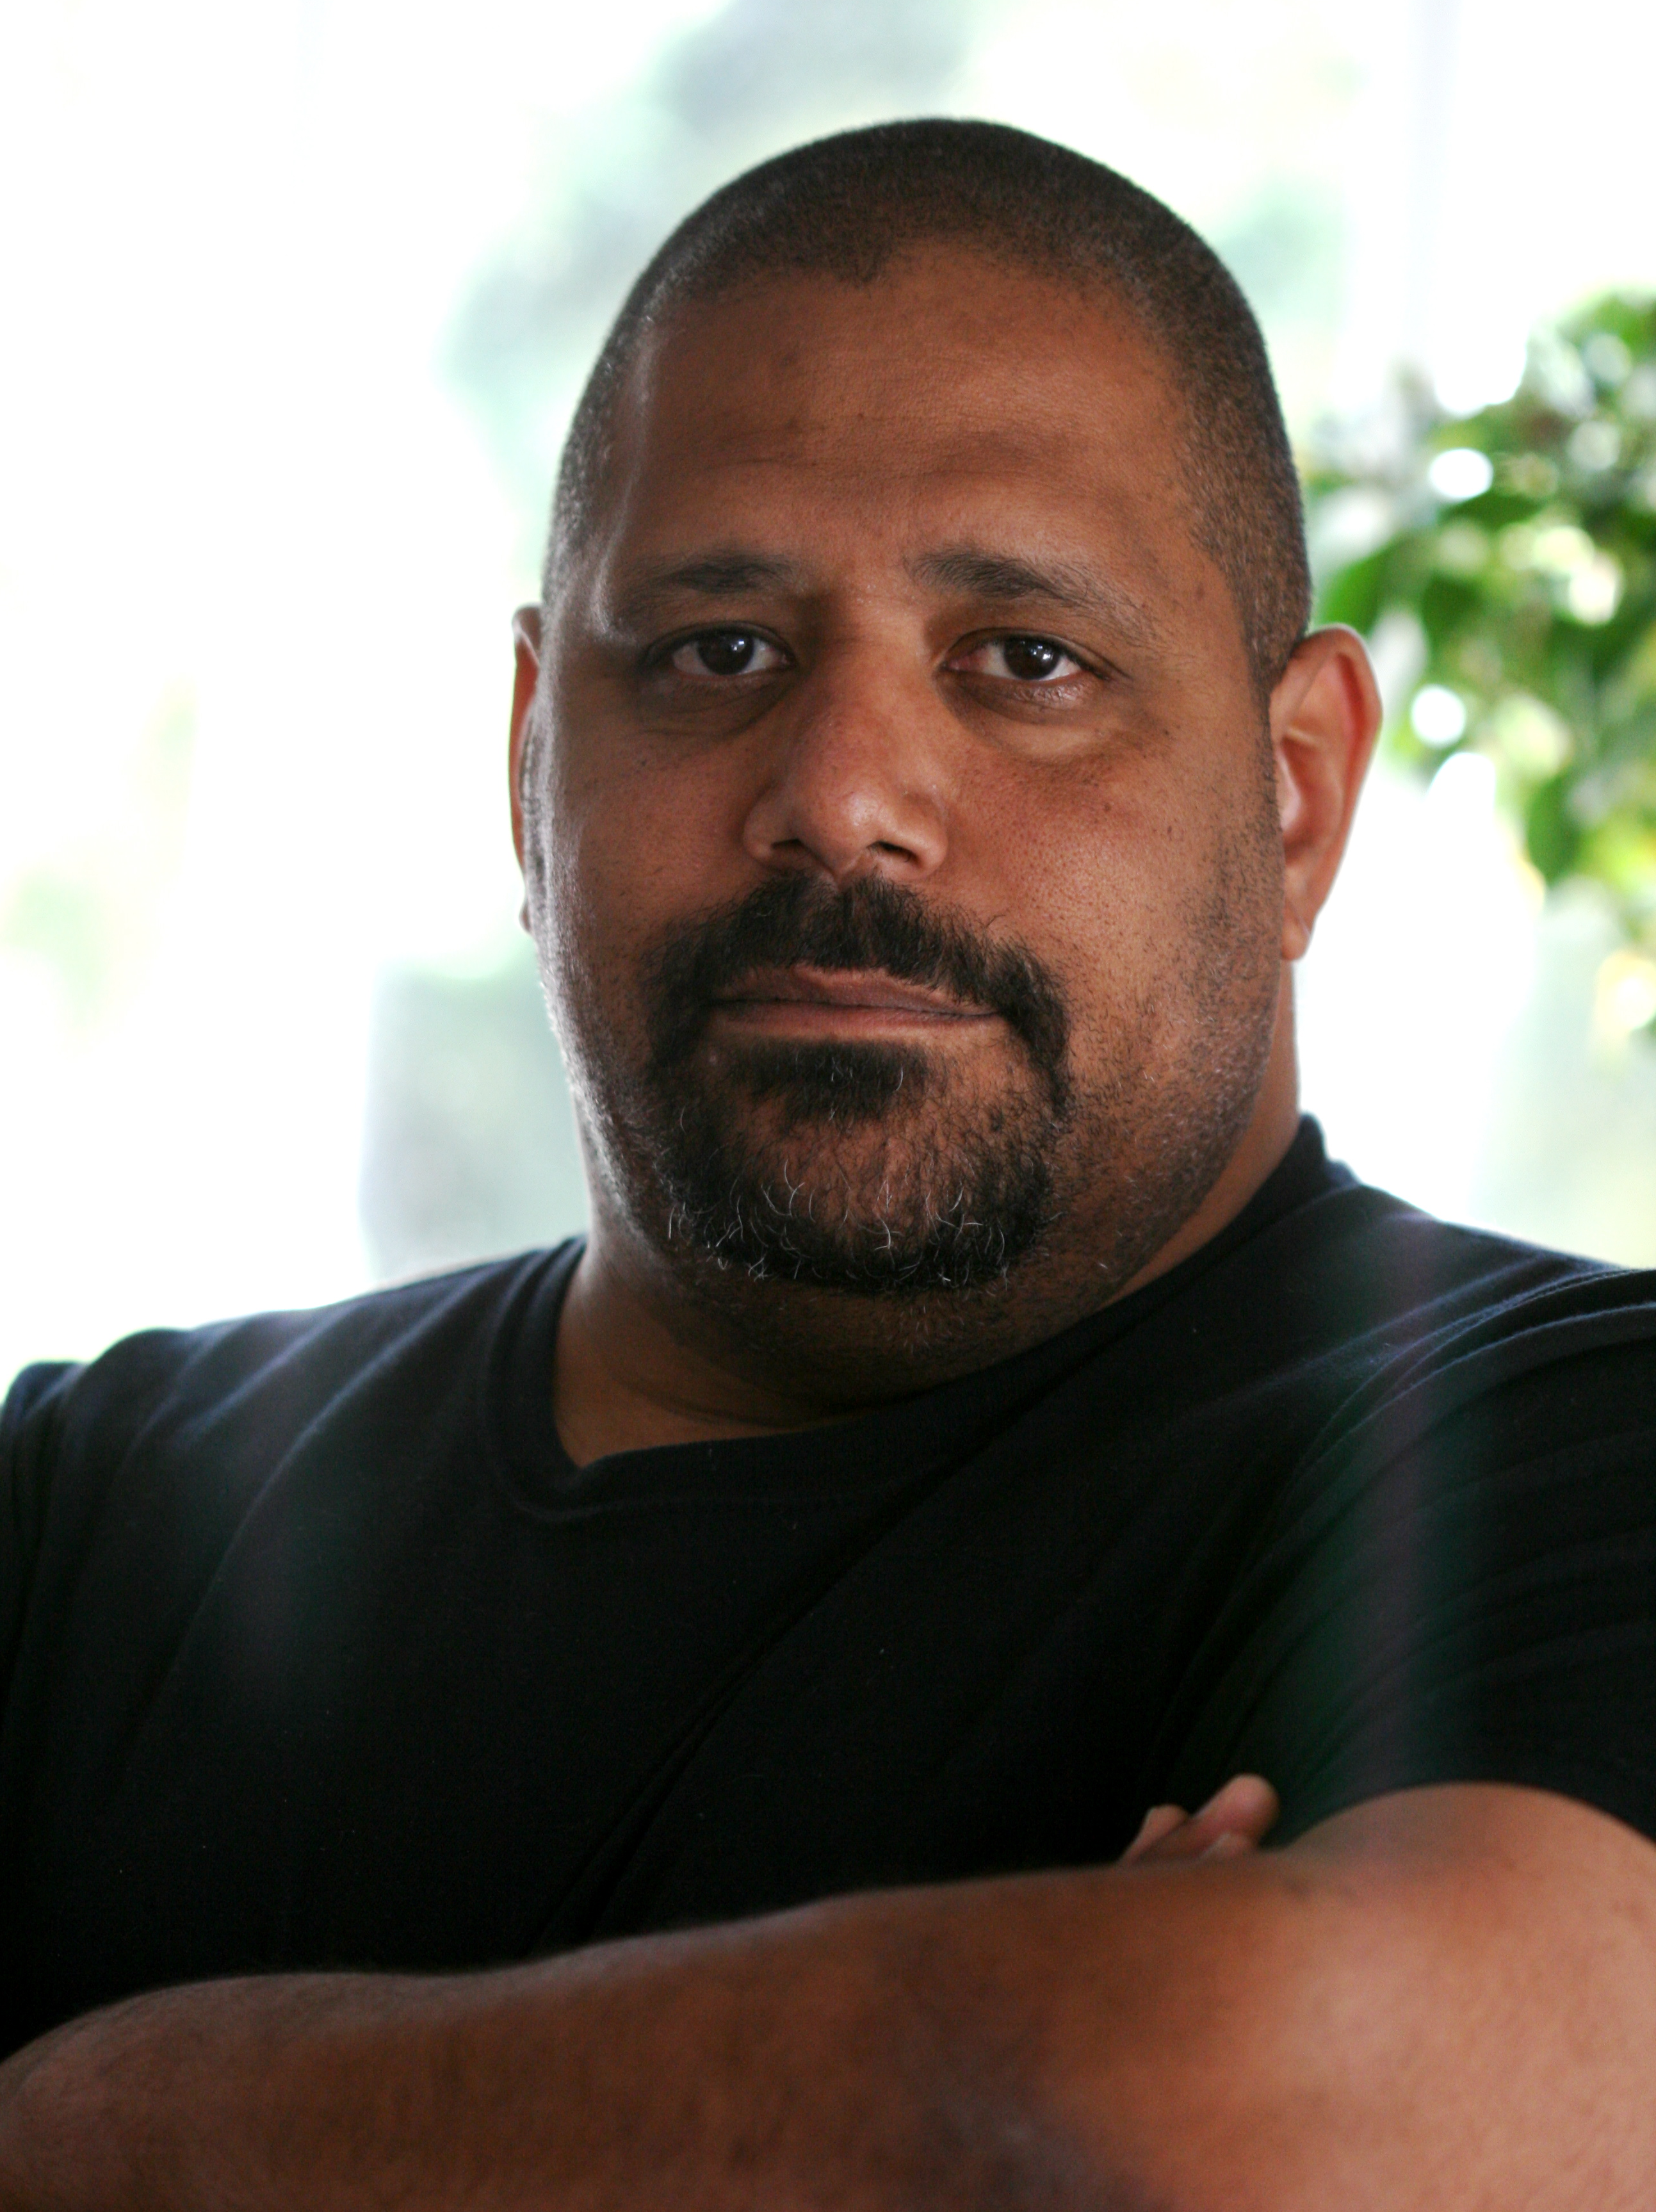
\includegraphics[scale=0.05]
    {./PresentationsPictures/OS-heroes-Pictures/Brian-J-Fox.png}

    \caption{Brian J.~Fox (ur.~1964). W~1989~r. stworzył powłokę
      \textsc{bash} (ang. \textit{Bourne-Again SHell}).}

    \label{fig:Brain-J-Fox}

  \end{figure}

\end{frame}
% ##################










% ######################################
\section{Maszyny, bo one też mają znaczenie}
% ######################################



% ##################
\begin{frame}
  \frametitle{Dalekopis (ang. \textit{teletypewriter})}


  \begin{figure}

    \centering


    \includegraphics[scale=0.6]
    {./PresentationsPictures/Machines-Pictures/Hughes-telegraph.jpeg}

    \caption{Dalekopis zaprojektowany przez Davida Edwarda Hughesa
      (1830-1900), wyprodukowany około 1855 roku.}

    \label{fig:Dalekopis-Hughesa}

  \end{figure}

\end{frame}
% ##################





% ##################
\begin{frame}
  \frametitle{Komputer PDP-7, lata 60-te XX wieku}


  \begin{figure}

    \centering


    \includegraphics[scale=0.2]
    {./PresentationsPictures/Machines-Pictures/PDP-7-with-teletype.jpeg}

    \caption{Komputer PDP-7 z~dalekopisem.}

    \label{fig:PDP-7-z-dalekopisem}

  \end{figure}

\end{frame}
% ##################





% ##################
\begin{frame}
  \frametitle{PDP-11, lata 70-te XX-wieku}


  \begin{figure}

    \centering


    \includegraphics[scale=0.225]
    {./PresentationsPictures/Machines-Pictures/PDP-11.jpeg}

    \caption{Komputer PDP-11.}

    \label{fig:PDP-11}

  \end{figure}

\end{frame}
% ##################





% ##################
\begin{frame}
  \frametitle{Dalekopis Teletype Model 33 ASR}


  \begin{figure}

    \centering


    \includegraphics[scale=0.028]
    {./PresentationsPictures/Machines-Pictures/Teletype-Model-33-ASR-01.jpeg}
    \includegraphics[scale=0.2]
    {./PresentationsPictures/Machines-Pictures/Teletype-Model-33-ASR-02.jpeg}

    \caption{Dalekopis Teletype Model~33 firmy Teletype Corporation,
      dostępny w~wersji komercyjnej od 1963~r. Jedna z~pierwszych urządzeń,
      które wspierało system kodowania ASCII. }

    \label{fig:Teletype-Model-33-ASR}

  \end{figure}

\end{frame}
% ##################










% ######################################
\section{W~jakich językach pisze~się systemy opearcyjne?}
% ######################################



% ##################
\begin{frame}
  \frametitle{W~jakich językach pisze~się systemy opearcyjne?}


  W~pewnym uproszczeniu, wszystkie pięć wielkich rodzin systemów
  operacyjnych, GNU/Linux, macOS, Windows, Android oraz iOS są napisane
  w~języku~C.

\end{frame}
% ##################








% ##################
\begin{frame}
  \frametitle{Kilka banalnych uwag na zakończenie}


  W~literaturze znajduje~się zarówno zapis „UNIX”, ale też i~„Unix”.
  Podobnie spotyka~się zarówno „MINIX” jak i~„Minix”, a~także warianty
  innych nazw. We~wszystkich tego typu przypadkach będę~się starał podążać
  za konwencjami używanymi w~książce Andrewa S. Tanenbauma \textit{Systemy
    operacyjne. Wydanie~III}
  \parencite{Tannenbaum-Systemy-Operacyjne-Wydanie-III-Pub-2013}, chyba
  że~względy estetyczne wymuszą użycie innej.

\end{frame}
% ##################





































% % ##################
% \begin{frame}
%   \frametitle{????}




% \end{frame}
% % ##################





% % ##################
% \begin{frame}
%   \frametitle{????}




% \end{frame}
% % ##################





% % ##################
% \begin{frame}
%   \frametitle{????}




% \end{frame}
% % ##################





% % ##################
% \begin{frame}
%   \frametitle{????}




% \end{frame}
% % ##################





% % ##################
% \begin{frame}
%   \frametitle{????}




% \end{frame}
% % ##################






% % ##################
% \begin{frame}
%   \frametitle{?????}




% \end{frame}
% % ##################





% % ##################
% \begin{frame}
%   \frametitle{?????}




% \end{frame}
% % ##################





% % ##################
% \begin{frame}
%   \frametitle{?????}




% \end{frame}
% % ##################





% % ##################
% \begin{frame}
%   \frametitle{?????}



% \end{frame}
% % ##################





% % ##################
% \begin{frame}
%   \frametitle{?????}



% \end{frame}
% % ##################





% % ##################
% \begin{frame}
%   \frametitle{?????}



% \end{frame}
% % ##################





% % ##################
% \begin{frame}
%   \frametitle{????}



% \end{frame}
% % ##################





% % ##################
% \begin{frame}
%   \frametitle{?????}



% \end{frame}
% % ##################





% % ##################
% \begin{frame}
%   \frametitle{????}



% \end{frame}
% % ##################





% % ##################
% \begin{frame}
%   \frametitle{?????}



% \end{frame}
% % ##################





% % ##################
% \begin{frame}
%   \frametitle{?????}



% \end{frame}
% % ##################





% % ##################
% \begin{frame}
%   \frametitle{????}



% \end{frame}
% % ##################





% % ##################
% \begin{frame}
%   \frametitle{????}



% \end{frame}
% % ##################





% % ##################
% \begin{frame}
%   \frametitle{?????}




% \end{frame}
% % ##################





% % ##################
% \begin{frame}
%   \frametitle{?????}




% \end{frame}
% % ##################





% % ##################
% \begin{frame}
%   \frametitle{?????}



% \end{frame}
% % ##################





% % ##################
% \begin{frame}
%   \frametitle{????}




% \end{frame}
% % ##################





% % ##################
% \begin{frame}
%   \frametitle{????}




% \end{frame}
% % ##################





% % ##################
% \begin{frame}
%   \frametitle{????}




% \end{frame}
% % ##################











% % ##################
% \begin{frame}
%   \frametitle{?????}





% \end{frame}
% % ##################





% % ##################
% \begin{frame}
%   \frametitle{????}




% \end{frame}
% % ##################
















% % ######################################
% \appendix
% % ######################################





% % ##################
% \endingslide???{}
% % ##################



% % % ##################
% % \jagiellonianendslide{?????}
% % % ##################





% ####################################################################
% ####################################################################
% Bibliography

\printbibliography





% ####################################################################
% End of the document

\end{document}
